The properties of an embedded 2DEG in the linear response regime under the influence of obstructions and changes in geometry are simulated. This section is partitioned into two parts. The first part examines the change of transport properties of a nano-wire when a constriction like a quantum point contact is introduced.\par
The second part investigates the 2DEG properties of systems of varying geometry and the possible implications of the knowledge of local electron and spin density.\par
\section{Colinear Quantum Point Contacts}

In chapter \ref{sec:conductancefromtransmission} the ``\emph{relation of conductance and transmission}'' \cite{landauer1996} was shown. The transmission of a device with a constriction ``small enough'' is \emph{quantized} as experiments have found out for semiconductor heterojunctions \cite{vanHoutenBeenakker2005} and metals \cite{PhysRevB.36.1284}. The analysis of quantized transmission merits the investigation of small constrictions in more detail.
The two-dimensional electron gas in a semiconductor heterojunction has a \textsc{Fermi} wavelength a hundred times larger than electrons in metal. This makes it possible to study constrictions with an opening comparable to the \textsc{Fermi} wavelength of $\sim 30\text{nm}$ and much smaller than the mean free path for impurity scattering. Constrictions like these are ``small enough'' and are called \emph{quantum point contacts} (QPC) \cite{vanHoutenBeenakker2005}. Because of the large \textsc{Fermi} wavelength these constrictions are \emph{mesoscopic} objects. That is an object on an intermediary scale between the microscopic and macroscopic domains.\par
The quantized nature of the conductance measurements is therefore highly dependent on the opening of the constriction. Not only on the transverse extent of the opening but also on the change of the \emph{potential landscape}, if adiabatic or abrupt,  around it \cite{PhysRevB.44.8017}. How the shape of the transmission function referred to as the \emph{conductance profile} is altered on changes of the confining potential landscape is subject of this section.\par
In the following different domains of potential change are illustrated. \Cref{fig:hardwalled} shows a \emph{hard walled} potential constriction with walls of infinite slope typical for example for devices etched out of a parent layer via reactive gases or the cleaved edge technique \cite{ApplPhysLett.66.323}. The adiabatic case is illustrated in \cref{fig:softwalled} by a constriction formed of two point charges. Here the potential landscape varies only slowly in any direction. A variational potential designed to investigate the dependence of certain 2DEG properties on the slope of the constricting potential is displayed in \cref{fig:variationalwalled}. Here the walls can be symmetrically modified to achieve different but constant slopes.
\begin{figure}[h!]
\begin{minipage}[c]{0.5\textwidth}
  \begin{tikzpicture}%[every text node part/.style={align=center}]
      \node at (0,0)[above] {\includegraphics[width=0.9\textwidth]{images/qpcrect-crop.png}};
      \axes
\draw[style={<->,thin}] ($1.125*(-1.3,3.6247)$) -- ($1.125*(-0.55,3.25)$) node[midway,left,yshift=-0.5em] {$d$};
\draw[style={<->,thin}] ($1.125*(0,2)$) -- ($1.125*(1,2.5)$) node[midway,above] {$w$};
    \end{tikzpicture}
    \end{minipage}
\begin{minipage}[c]{0.5\textwidth}
 \begin{flalign}\quad\text{Pot}(x,y) =\ &\Theta(d/2-\abs{x})&\notag\\
 \cdot\ &\Theta(\abs{y}-w/2)&\end{flalign}
 \end{minipage}
\caption{Potential landscape of hard-walled QPC. Here $x$ is the longitudinal direction of electron flow and $y$ the transverse. $d$ denotes the depth of the wall and $w$ the width of the opening }\label{fig:hardwalled}
\end{figure}
\begin{figure}[h!]
% \begin{tabularx}{\textwidth}{m{0.45\textwidth} m{0.55\textwidth}}
\begin{minipage}[c]{0.5\textwidth}
  \begin{tikzpicture}%[every text node part/.style={align=center}]
      \node at (0,0)[above] {\includegraphics[width=0.9\textwidth]{images/qpcpoint-crop.png}};
      \axes
\draw[style={<->,thin}] ($1.125*(-1.6,3)$) -- ($1.125*(1.3,4.3)$) node[midway,above] {$w$};
    \end{tikzpicture}
    \end{minipage}
\begin{minipage}[c]{0.5\textwidth}
 \begin{flalign}\quad\text{Pot}(x,y) &= \frac{q}{\sqrt{x^2+(y+w/2)^2}}&\notag\\
 &+\frac{q}{\sqrt{x^2+(y-w/2)^2}}&\end{flalign}
    \end{minipage}
% \end{tabularx}
\caption{Potential landscape of soft-walled QPC of two point charges. Re-normalized field of two point charges of charge $q$ and dislocation $w$.}\label{fig:softwalled}
\end{figure}
% \begin{figure}[h!]
%   \begin{minipage}[c]{0.5\textwidth}
%   \begin{tikzpicture}%[every text node part/.style={align=center}]
%       \node at (0,0)[above] {\includegraphics[width=.9\textwidth]{images/qpcvariational-crop.png}};
%       \axes
% % \draw[style={-,thin}] (2,0.65) -- (2,1.3) node[midway,above] {$w$};
% % \draw [help lines] (0,0) grid (3,3);
%   \coordinate (a) at ($1.125*(1.05,1.62)$);
%   \coordinate (b) at ($1.125*(1.75,2.015)$);
%   % \coordinate (c) at ($(b)+(-0.2,1.322)$);
%   \coordinate (c) at ($1.125*(1.75,3.582)$);
%   \coordinate (d) at ($1.125*(0.21,2.05)$);
%   \coordinate (e) at (0.0506,2.508);
%   \coordinate (f) at (0.73,4.5);
%   \draw[-] (a) node[above,yshift=2em]{$m$} -- (b) node[midway,below,xshift=0.8em]{$\Delta y$} -- (c) --cycle;
%   \draw[dashed] (a) -- (d);
%   \draw[-] (e) -- (f);
%   \draw[dashed] (c) -- (f);
%     \end{tikzpicture}
% \end{minipage}
% \begin{minipage}[c]{0.5\textwidth}
% \begin{flalign}\quad\text{Pot}(x,y) &= e^{-x^2/\xi^2}\cdot\abs{m\cdot y}&\end{flalign} 
% \end{minipage}
% \caption{Example potential landscape of variational-walled QPC used in analysis}\label{fig:variationalwalled}
% \end{figure}
\begin{figure}[h!]
  \begin{minipage}[c]{0.5\textwidth}
  \begin{tikzpicture}%[every text node part/.style={align=center}]
      \node at (0,0)[above] {\includegraphics[width=.9\textwidth]{images/qpcvariational2-crop.png}};
\draw[style={<->,thin}] ($1.125*(-0.205,2)$) -- ($1.125*(0.27,2.25)$) node[midway,above] {$w$};
      \axes
  \coordinate (a) at (1.65,2.3);
  \coordinate (b) at (2.6,2.87825);
  % \coordinate (b) at (2.505,2.81325);
  \coordinate (c) at (2.6,3.982);
  \coordinate (e) at (0.53,2.9);
  \coordinate (f) at (1.45,4.5);
  \draw[-] (a) node[above,xshift=0.5em,yshift=2em]{$m$} -- (b) node[midway,below,yshift=0.3em,xshift=0.8em]{$\Delta y$} -- (c) --cycle;
  \draw[dashed] (a) -- (e);
  \draw[-] (e) -- (f);
  \draw[dashed] (c) -- (f);
    \end{tikzpicture}
\end{minipage}
\begin{minipage}[c]{0.5\textwidth}
\begin{flalign}\quad\text{Pot}(x,y) &= e^{-x^2/\xi^2}\cdot m(\abs{y}- w/2)&\end{flalign} 
\end{minipage}
\caption{Example potential landscape of variational-walled QPC used in analysis.The slope of the transverse confinement is given by $m$ and the width at the bottom of the opening by $w$.The parameter $\xi$ controls the steepness of the walls in $x$ direction.}\label{fig:variationalwalled}
\end{figure}
The presented QPCs serve only as examples for three classes of constrictions. A sample of constrictions of different geometry are considered for each class in the following. The simulations sweeps either the geometrical opening of the constriction or the energy domain, which is equivalent for example for the QPC formed by point charges. Modifying the width of the QPC opening is usually experimentally achieved by the placement of several gate electrodes on or in the 2DEG on a negative potential effectively depopulating the conductance band in their vicinity. The width of the constriction can either be directly geometrically modified ore for the case of the point charges via the charge $q$. It is important to note that by changing the voltage on the electrodes and therefore the charge not only the width of the opening is changed but also the steepness of the confining potential for a given energy. The transfer from the adiabatic to the diabatic i.e steep walled domain is possible.\par
The simulation is set up that electrons with a wavevector pointing in the direction of the constriction are placed in the lead at the top of all density plots corresponding to the linear response regime of transport.
For all presented quantum point contacts, some sketched in \cref{fig:hardwalled,fig:variationalwalled}, the width of the constriction is varied for a fixed energy of $E=0.06t_0$ corresponding to 15 modes within the unconstriced wire of 200nm width. A lattice spacing of a=1nm, and an effective mass of $0.026 \times m_0$ as in \cref{sec:validation}. The \textsc{Rashba} parameter is set to a typical value of $\alpha = 20^{-12}$eVm\,\cite{Jacob2009Thesis}.
\subsubsection{Hard-Walled QPCs}
\todo[noline]{translate all transmission plots to 'width'}The general geometry of quantum devices embedded in 2DEGs prepared by etching commonly exhibits steep walls of the confining potential. Thus the influence of unbiased geometrical constrictions on the transport properties of the 2DEG are considered first.
\begin{figure}[h]
\subfloat[Edens]{\label{fig:rectedens}\includegraphics[]{images/238916-wire400x200-Nov-28-2011-17.41edens}}
\subfloat[Spindens]{\label{fig:rectspindens}\includegraphics[]{images/238916-wire400x200-Nov-28-2011-17.41spindens}}
\caption{Simulated electron and spin density of a rectangular QPC opening. Snapshot of constriction width=100nm,$d=60nm$}
\end{figure}
A constriction similar to the \emph{rectangular} discontinuous potential shown in \cref{fig:hardwalled} is used as a starting point of the analysis of 2DEGs with QPCs.\par
The electron density shown in \cref{fig:rectedens} shows the expected formation of modes within the constriction. In the areas towards the leads however strong interference possibly from backscattering disturbs the establishment of continuous electron flux tubes. The spin density in \cref{fig:rectspindens} shows a similar comlex interference pattern as the electron density. Interestingly two areas of dominant upward polarization to the left and downward polarization to the right side of the constriction is present. This effect seems related to the diffusion of spin injection from the QPC into the lead.\par
\begin{figure}[h]
\centering
\includegraphics[]{images/238916-wire400x200-Nov-28-2011-17.41trans}
\caption{Simulated transmission profile}
\end{figure}
In the conductance plot very distinct steps of height 2 are visible corresponding to one conductance quantum per mode per spin up and spin down electron. The diminished spin degeneracy is responsible for the irregularities around the steps and will be shown in detail for a QPC conductance exhibiting a more pronounced effect in one of the following simulations.\par
\begin{figure}[h]
\subfloat[Edens]{\label{fig:triedens}\includegraphics[]{images/wire400x200-Nov-28-2011-00.47edens}}
\subfloat[Spindens]{\label{fig:trispindens}\includegraphics[]{images/wire400x200-Nov-28-2011-00.47spindens}}
\caption{Simulated electron and spin density for triangle shaped constriction tip. Snapshot corresponds to an opening of ???}
\end{figure}
To remedy the abrupt potential change a \emph{triangular} potential is introduced. If thought of as the tip of an electrode this geometry comes close to the physical  shape of the constriction used by \textsc{Wees} et. al \cite{PhysRevLett.60.848}. As expected the electron flow shows more continuous densities in \cref{fig:triedens}. There also appear a number of points of high electron density in the upper and lower part due to the reflections of the perpendicular QPC wall.\par
\begin{figure}[h]
\centering
\includegraphics[]{images/wire400x200-Nov-28-2011-00.47trans}
\caption{Simulated transmission profile}\label{fig:tritrans}
\end{figure}
In the spin density plot in \cref{fig:trispindens} a spin split pattern very similar to the rectangular case can be observed. The spin down electrons and spin up electrons will be separated after passing the constriction but there exists a more complex interaction pattern along the central axis in $y$ direction of the wire.Additionally the regularity of almost parallel spin split in the very ends of the device is diminished. These effects might explain the unexpected result of the conductance quantization or the lack thereof.
It is interesting to note that there are almost no steps visible in \cref{fig:tritrans} although the situation is actually "more adiabatic" because of the angled change in $x$ direction as is obvious by observing the continuous lines of electron density within the constriction. For low intrusion of the QPC tips rather smooth steps of height 2 can be seen. A smoother shape is expected for devices with less abrupt changes but the tips still present \emph{infinite} walls. A possible non-physical cause might lie in the discretization. Because the device is mapped on a square lattice the angled walls of the constriction become highly ragged. This series of longitudinal and transverse wall segments might give rise to a steep increase of scattering effectively smoothing out the conductance steps due to a higher spread in the kinetic energy distribution of the propagating electrons.
% \begin{figure}[h]
% \subfloat[Edens]{\includegraphics[]{images/}}
% \subfloat[Spindens]{\includegraphics[]{images/}}
% \caption{Simulated electron and spin density}
% \end{figure}
% \begin{figure}[h]
% \centering
% \includegraphics[]{images/}
% \caption{Simulated transmission profile}
% \end{figure}
\FloatBarrier
\subsubsection{Soft-Walled QPCs}
The geometrical shape of the constriction influences the transport properties of the device as seen in the previous section. Changing the geometry perpendicular to the $z$-axis smoothed out most features related to quantized conductance either physically or by introducing artificial complexity not found in the actual continuous system.\par
One possible remedy is to alter the slope of the confining potential landscape perpendicular to the $x$ and $y$-axis. This stands in opposition to the infinite slope of the hard walled potentials considered before. A potential wall slowly varying in respect to the $x$ and $y$ coordinates will be called \emph{soft walled}.\par
\begin{figure}[h]
\subfloat[Electron density $n$]{\label{fig:sphericaledens}\includegraphics[]{images/wire400x200-Nov-27-2011-21.41edens}}
\subfloat[Spin density in measures of $\hbar/m^2$]{\label{fig:sphericalspindens}\includegraphics[]{images/wire400x200-Nov-27-2011-21.41spindens}}
\caption{Simulated electron and spin density of a 2DEG with spherical constriction.}
\end{figure}
The \emph{spherical} electrode tip is a shape with characteristics of both infinite wall and adiabatically varying potential walls. The hard walls perpendicular to each lateral axis are gradually smoothed towards higher potential. The rectangular or triangular tip of the gate electrodes are replaced by a quarter-circle which for small intrusions mimics the potential introduced by a top gate above the 2DEG. Looking at the electron density in \cref{fig:sphericaledens} a resemblance to the prior tip shapes can be seen. The structure exhibits the increased continuous electron densities as well as points of high electron densities symmetrically arranged in the upper and lower half similar to the triangular tip. Also the spin densities in \cref{fig:sphericalspindens} only differ slightly from the triangular case.\par
\begin{figure}[h]
\centering
\includegraphics[]{images/wire400x200-Nov-27-2011-21.41trans}
\caption{Simulated transmission profile}
\end{figure}
Despite the similarities to the triangular case clearly pronounced steps are seen in the conductance profile. The variations near the steps are smoothed out without the loss of discrete steps of height 2. Because of these characteristics it is used to validate the results of the conductance calculations in section \ref{sec:validation}.\par
\begin{figure}[h]
\subfloat[Electron density $n$ for the 2DEG constrained in the $y$ direction by two point charges.]{\label{fig:pointedens}\includegraphics[]{images/242255-wire400x200-Dec-02-2011-23.08edens}}
\subfloat[Spin density $s_z$ of the 2DEG constrained in the $y$ direction by two point charges.]{\label{fig:pointspindens}\includegraphics[]{images/242255-wire400x200-Dec-02-2011-23.08spindens}}
\caption{Simulated electron and spin density for a constriction formed by two point charges c.f.~\cref{fig:softwalled}. The point charges are located at the transverse boundary of the wire 200nm apart. Snapshot corresponds to $q\approx 1.5\cdot 10^{-18}$ C}
\end{figure}
In the following simulation point charges were introduced in the vicinity of the 2DEG to model a constriction formed by gate electrodes more closely. A QPC of this kind exhibits a very slow varying potenital throughout large parts with almost infinite slopes near the location $r_q$ of the point charges due to the $\sim 1/r_q$ dependency.\par
The electron density pictured in \cref{fig:pointedens} show the expected continuous flux tube at the very edge of the nano-wire while the center region is subject to complex interference. An interference pattern can also be seen in before and after the QPC although much simpler in comparison to all prior QPCs. The lateral offset near the upper and lower lead are due to the necessity to cut off the potential at some point which would otherwise extend to infinity.
Although the maximum spin splitting is lower compared to all prior QPCs it exhibits a much simplified interference pattern with highly localized areas of maximum polarization and otherwise almost negligible polarization. The simplicity is due to the reduced number of modes. The probability distribution of the electrons is laterally confined to the same area but because of the slow decrease of the potential there exists a finite potential throughout the device.\par
\begin{figure}[h]
\centering
\includegraphics[]{images/242255-wire400x200-Dec-02-2011-23.08trans}
\caption{Simulated transmission profile of QPC of two point charges for a spin degenerate system}\label{fig:qpcpointnospin}
\end{figure}
Similar to the twofold nature of the densities characteristics of both steep walled an adiabatic potentials can be found in the conductance profile, \cref{fig:pointtrans}. For one a well pronounced first and second conductance step can be seen but on the other hand the steps smooth out more the lower the charge. Interestingly the steps become well pronounced again when the charge approaches zero. As this pattern is also observed for spin degenerate systems as can be seen in \cref{fig:qpcpointnospin} a relation of this effect to a spin-orbit coupling seems unlikely. 
The disappearance of steps can be accounted for with the onset of \emph{inter-subband scattering} which have been observed to have significant effect starting at the fourth mode \cite{Lehmann2011}. If inter-subband scattering is indeed the cause for the smoothing of the conductance profile the re-appearance of noticeable steps would correspond to the reduction of inter-subband scattering due to some change in the device at lower charge.
Note that as the charge decreases the steepness of the potential increases for a given electron energy $E_{e^-}$ as is illustrated in \cref{fig:differentq}.
The only obvious change in the 2DEG at lower charge is the height and steepness of the potential landscape. To investigate the relation of the steepness of the potential landscape to the diminishing conductance quantization a parametrized  QPC pictured in \cref{fig:variationalwalled} is introduced into the 2DEG.
\begin{figure}[h] 
\centering
\subfloat[Simulated conductance profile.]{\includegraphics[]{images/242368-wire400x200-Dec-03-2011-04.35trans}}
\subfloat[Transverse potential profile in Volt at different charge $q_1 = 6.5 \cdot 10^{-18}$C and $q_2= 1 \cdot 10^{-18}$C.]{\label{fig:differentq}\includegraphics{images/differentq}}
\caption{Conductance profile and sample of confining potential at different charge.}\label{fig:pointtrans}
\end{figure}
\FloatBarrier
\subsubsection{Variational-Walled QPCs}
The effects of wall slope on the smoothness of the conductance profile and thus possibly on inter-subband scattering are investigated by increasing the width of the constriction for many different slopes $m$. Above a slope of $m \approx 0.03$ the conduction shows quantized steps of conduction with no significant effects if the slope changes in that interval. For slowly varying potential slopes a noticeable change in conduction quantization can be observed as can be seen in \cref{fig:slopes}. \Cref{fig:conductances} shows conductance profiles at constant slopes. A significant change in quantization is only seen in the slope-interval $0.008 \lt m \lt 0.032$.\par
The electron densities in \cref{fig:variedens1} and \cref{fig:variedens2} provide further indications of inter-subband scattering. The comparison shows that the electron density for the softer QPC is much less localized in discrete channels. This could indicate an increase in interaction of the modes passing through the QPC.\par
\begin{figure}[h] 
\centering
\subfloat[Conductance profiles for different slopes $m$]{\label{fig:slope_cuts}\includegraphics[]{images/slope_cuts.pdf}}
\subfloat[Full conductance profile for QPC opening sweep. Plotted is the conductance of the QPC for different width $w$ and transverse steepness $m$ of the constriction]{\label{fig:slopes}\includegraphics[width=0.5\textwidth]{images/slopes.png}}
\caption{Conductance profiles at different slopes and full conduction profile slope vs. width.}\label{fig:conductances}
\end{figure}
Interestingly the spin split is increased for the smoother walled QPC in \cref{fig:varispindens1} in comparison to \cref{fig:varispindens2} and most other investigated constriction shapes. Additionally it exhibits less dominant interference features than any hard walled potential what is to be suspected as the smoother the potential landscape the less likely is a reflection that alters the trajectory significantly.\par
There seem to be strong indications for the interaction of wall slope and possible inter-subband scattering similar to the mixing of intra-subband eigenstates due to higher order effects of the \textsc{Rashba} spin-orbit interaction \cite{Wolfgang2003PhysicaE.18.337}. Spin-orbit coupling influenced by the shape of the constriction could also explain the difference in spin-polarization and could be subject to further analysis.
\begin{figure}[h]
\subfloat[Electron density $n$ for the 2DEG.]{\label{fig:variedens1}\includegraphics[]{images/1edens}}
\subfloat[Spin density $s_z$ of the 2DEG.]{\label{fig:varispindens1}\includegraphics[]{images/1spindens}}
\caption{Simulated electron and spin density for a constriction formed by a variational-walled constriction of slope $m=0.008$. Snapshot corresponds to a conductance of 16$e^2/h$}
\end{figure}
\begin{figure}[h]
\subfloat[Electron density $n$ for the 2DEG.]{\label{fig:variedens2}\includegraphics[]{images/4edens}}
\subfloat[Spin density $s_z$ of the 2DEG.]{\label{fig:varispindens2}\includegraphics[]{images/4spindens}}
\caption{Simulated electron and spin density for a constriction formed by a variational-walled constriction of slope $m=0.032$. Snapshot corresponds to a conductance of 16$e^2/h$ }
\end{figure}
\FloatBarrier
\section{Non-Colinear devices}
Changes in the geometry of the device can be made to exploit the knowledge of local properties of the 2DEG. Due to the symmetrical nature of the spin-plit breaking the symmetry of the system introduces new effects. To that end the assumption of colinear leads has to be dropped. A simple bend in the nano-wire already introduces complex interactions in real-space as well as spin-space. This is demonstrated in \cref{fig:curvedens1,fig:curvedens2,fig:curvedens3,fig:curvspindens1,fig:curvspindens2,fig:curvspindens3}. The first three modes correspond respectively to the energies 0.003eV, 0.036eV and 0.081eV of a straight nano-wire of same width. If compared to \cref{fig:dens1,fig:dens2,fig:dens3} for example an apparent change is immeadiatlely seen. Not only is the spacial distribution of electrons along the wire not constant but the spin densities exhibit a preference for up polarized electrons. Note that the scales change about the order of 2 to prevent the loss of details for smaller spin-split and electron densities. The features of the curved 2DEG are highly energy dependent and only serve to illustrate the enhanced complexity of non-colinear geometry.
\begin{figure}[h!]
\subfloat[Electron density of first mode in curved nano-wire. $E_{mode}=0.003$eV.]{\label{fig:curvedens1}\includegraphics[]{images/curve_1modes_edens}}
\subfloat[Electron density of second mode in curved nano-wire. $E_{mode}=0.036$eV.]{\label{fig:curvedens2}\includegraphics[]{images/curve_2modes_edens}}
\subfloat[Electron density of third mode in curved nano-wire. $E_{mode}=0.081$eV. ]{\label{fig:curvedens3}\includegraphics[]{images/curve_3modes_edens}}
\caption{Electron densities for a curved nano-wire of 40nm width. Because of the bend the wire-width is marginally reduced in the curve. Colour indicates electron density. The density increases from Blue=0 to Red=Max($n$).}
\end{figure}
\begin{figure}[h!]
\subfloat[Spin density of first mode in curved nano-wire.  $E_{mode}=0.003$eV.]{\label{fig:curvspindens1}\includegraphics[]{images/curve_1modes_spindens}}
\subfloat[Spin density of second mode in curved nano-wire. $E_{mode}=0.036$eV.]{\label{fig:curvspindens2}\includegraphics[]{images/curve_2modes_spindens}}
\subfloat[Spin density of third mode in curved nano-wire. $E_{mode}=0.081$eV.]{\label{fig:curvspindens3}\includegraphics[]{images/curve_3modes_spindens}}
\caption{Spin densities for a curved nano-wire of 40nm width. Because of the bend the wire-width is marginally reduced in the curve. Colours indicate spin polarization. Red=Up, Blue=Down.}
\end{figure}
A common approach to the manipulation of properties of wave objects is an interferometer. A simple realization of such an interferometer can be realized as a modification of the \textsc{Arahonov-Bohm} ring. The \textsc{Arahonov-Bohm} ring is a two-dimensional annulus with a radius larger than separation of the concentric circles. Spin interference has been achieved via the attachment of multiple leads \cite{PhysRevB.75.035304} or the application of an electro-magnetic field \cite{PhysRevB.69.155335} to the \textsc{Arahonov-Bohm} ring.\par
\begin{figure}[!h]
\centering
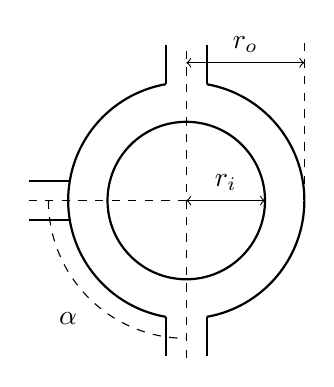
\begin{tikzpicture}
  % \draw[step=.5cm,gray,very thin] (-2,-2) grid (2,2);
  % \draw[dashed] (1.5,0) -- (1.5,0);
  \draw[dashed] (0,-2) -- (0,2);
  \draw[dashed] (0,-2) -- (0,2);
  \draw[dashed] (0,0) -- (-2,0);
  % \draw[dashed] (1,0) -- ++(0,1.5);
  \draw[dashed] (1.5,0) -- ++(0,2);
  \draw[<->] (0,1.75) -- node[above] {$r_o$}++(1.5,0);
  \draw[<->] (0,0) -- node[above] {$r_i$}++(1,0);
  \draw[dashed] (-1.75,0) arc (0:90:-1.75);
  \node (a) at (-1.5,-1.5) {$\alpha$};
  \draw[thick] (0,0) circle (1);
  \draw[thick] (1.5,0) arc (0:80:1.5) coordinate (n1);
  \draw[thick] (-1.5,0) arc (0:-80:-1.5) coordinate (n2);
  \draw[thick] (n1)-- ++(0,0.5);
  \draw[thick] (n2)-- ++(0,0.5);
  \draw[thick] (1.5,0) arc (0:-80:1.5) coordinate (n3);
  \draw[thick] (-1.5,0) arc (0:80:-1.5) coordinate (n4);
  \draw[thick] (n3)-- ++(0,-0.5);
  \draw[thick] (n4)-- ++(0,-0.5);
  \draw[thick] (-2,0.25)-- ++(0.51,0);
  \draw[thick] (-2,-0.25)-- ++(0.51,0);
\end{tikzpicture}
\caption{\textsc{Aharonov-Bohm} ring based interferometer of inner radius $r_i=65$nm and outer radius $r_o=75$nm. The angle $\alpha$ denotes the rotation of the lower lead to the upper lead. Here $\alpha=\pi/2$}\label{fig:aharonovbohmring}
\end{figure}
The most basic interferometer is achieved by the attachment to of two leads to the \textsc{Aharonov-Bohm} ring. To investigate changes in spin properties of the 2DEG one of the leads is then rotated against the other to obtain different enclosed angles. The device and process is sketched in \cref{fig:aharonovbohmring}.
\begin{figure}[h!]
\subfloat[Electron density $n$. Enclosing angle $\alpha=0$.]{\label{fig:ring0edens}\includegraphics[]{images/ring0edens}}
\subfloat[Electron density $n$. Enclosing angle $\alpha=\pi/2$.]{\label{fig:ring90edens}\includegraphics[]{images/ring90edens}}
\subfloat[Electron density $n$. Enclosing angle $\alpha=-\pi/2$.]{\label{fig:ringneg90edens}\includegraphics[]{images/ringneg90edens}}
\caption{Electron densities in \textsc{Aharonov-Bohm} type ring for three different enclosing angles. Color denotes density, Blue=0, Red=Max($n$).} 
\end{figure}
\begin{figure}[h!]
\subfloat[Spin density $s_z$. Enclosing angle $\alpha=0$.]{\label{fig:ring0spindens}\includegraphics[]{images/ring0spindens}}
\subfloat[Spin density $s_z$. Enclosing angle $\alpha=\pi/2$.]{\label{fig:ring90spindens}\includegraphics[]{images/ring90spindens}}
\subfloat[Spin density $s_z$. Enclosing angle $\alpha=-\pi/2$]{\label{fig:ringneg90spindens}\includegraphics[]{images/ringneg90spindens}}
\caption{Spin densities in \textsc{Aharonov-Bohm} type ring for three different enclosing angles. Color denotes spin polarization. Blue=Down, Red=Up}
\end{figure}
The interference of spin is already for colinear leads well pronounced. The polarization is in contrast to a wire or closed ring \cite{PhysRevB.82.165322} dependent on angular coordinate $\phi$.
The spins interact to form a standing wave in steady state. The circumference of a concentric circle in the center of inner and outer circle is $\approx 408$nm. For this energy of (???) 23 peaks and troughs of the standing wave can be counted, corresponding to a wavelength of $\lambda_{\text{spin}}=17.75$nm. This length is well below the spin-precession length in undisturbed geometries of $\approx230$nm for the parameters of this 2DEG.\par
Upon rotation of the lower lead the interference pattern changes considerably in amplitude and spatial profile. The phase of the standing wave appears to be fixed to the bottom lead and rotates the peaks and troughs according to the angle the lead has been rotated. Whereas the polarization in the leads is almost negligible throughout \cref{fig:ring0edens,fig:ring90edens,fig:ringneg90edens,fig:ring0spindens,fig:ring90spindens,fig:ringneg90spindens} the amplitude increases sharply within the ring. The amplitudes of spin polarization within the \textsc{Aharonov-Bohm} ring with rotated lead decrease gradually with increasing rotation in about one order of magnitude.\par
For the presented angles of 0,$\pi/2$ and $-\pi/2$ three very distinct situations occur. While the spin up to spin down amplitude ratio is unity for the symmetric device in \cref{fig:ring0edens} it reaches $n_{\uparrow}/n_{\downarrow}=5$ for $\alpha=\pi/2$ rotation in \cref{fig:ring90edens} and $n_{\uparrow}/n_{\downarrow}=0.2$ for $\alpha=-\pi/2$ rotation in \cref{fig:ringneg90spindens}. The electron densities in the ring with rotated leads are about twice as large in the longer arms than the shorter arms what is probably at least in part correlated to the increase in spin density.\par
Qualitatively this result is reproduced analytically for a one dimensional ring for the presented rotations. Solving the \hamil{} for closed ring in polar coordinates one obtains the four eigenstates in each arm \cite{nitta1999.695}:
\begin{align}
\Psi^{\pm}_{\uparrow} = e^{i\phi}\begin{pmatrix}\text{cos}(\theta/2)\\\pm\text{sin}(\theta/2)e^{i\phi}\end{pmatrix} 
\qquad\text{and}\qquad
\Psi^{\pm}_{\downarrow} = e^{\pm i\phi}\begin{pmatrix}\pm\text{sin}(\theta/2)e^{-i\phi}\\-\text{cos}(\theta/2)\end{pmatrix}
\end{align}
Plus and minus denotes the direction of travel and $\uparrow,\downarrow$ spin up and spin down respectively. Expanding each wave function in terms of the eigenstates the interference pattern in \cref{fig:ring90spindens} for example can be reproduced assuming partial reflection of the spin up wave function and total transmission of the spin down wave function at the junctions in the right arm and partial reflection of both spin states at the junctions in the left arm. 
\begin{figure}[!h]
\centering
\includegraphics[scale=0.5]{images/spinors}
\caption{Expansion of spin states in eigenstates of the closed ring. Negative $\phi$ corresponds to the left arm and positive $\phi$ to the right.}
\end{figure}
For enclosing angles not an integer multiple of $\pi/2$ this model breaks down quickly. Due to the finite spin polarization within the lead the isolated eigenstates of the closed ring do not give an accurate model of the physical situation.
